%!TEX root = ../article.tex

The goal of this section is to prove Theorem \ref{thm:detailed} part \ref{pa:construct} and the ``if" direction of parts \ref{pa:dualprojs} and \ref{pa:principalprojs}.   Thus we explicitly construct certain rational forms and determine when they are complete.  These constructions all follow quickly from the generators and relations presentation of the `Haagerup subfactor planar algebra' $\cH_0$ (from \cite{0902.1294}) and of the `extended Haagerup subfactor planar algebra' $\cH_1$ (from \cite{0909.4099}).   We modify these previous constructions slightly by using the lopsided normalization for cups and caps instead of the spherical one.  Furthermore, we have rescaled the generator: our $S$ is $\lambda_\ell$ times the $S$ of \cite{0909.4099, 0902.1294}.  (Both of these modifications were made in order to simplify the numbers that appear in the definition so that they lie in a smaller field.)

Let $\ell=0$ or $1$, and let $n=4\ell+4$.  Choose $q$ so $q+q^{-1}=\sqrt{D_\ell}$, and define the quantum integers as usual by $[m]=\frac{q^m - q^{-m}}{q-q^{-1}} \in \Integer[\sqrt{D_\ell}]$ (so in particular, $[2] = \sqrt{D_\ell}$).  
If $m$ is odd then $[m] \in \Rational(D_\ell)$.  If $m$ is even, then $[2][m] = [m+1]+[m-1]\in \Rational(D_\ell)$, and also any ratio of two even quantum integers lies in $\Rational(D_\ell)$.  We will write $\check{r} = \frac{[n+2]}{[n]} \in \Rational(D_\ell)$ throughout. (This number is the ratio of Perron-Frobenius dimensions of the two vertices past the branch point on the dual principal graph. The corresponding ratio on the principal graph is just $1$.)

Define $\lambda_\ell = [2]^{-1}\sqrt{-\check{r}}$ (these are the same as the explicit numbers given in the introduction) and note that $\lambda_\ell^2 = - \frac{[n+2]}{[2]^2[n]} \in \Rational(D_\ell)$. 
%Further, \todo{Why is $d_\ell^2 \in \Rational(\lambda_\ell)$?} 
Since $\lambda_\ell^2$ is not rational, and the degrees $[\Rational(D_\ell):\Rational]$ are prime, it follows that $\Rational(D_\ell) = \Rational(\lambda_\ell^2)$, and in particular 
$\Rational(D_\ell) \subset \Rational(\lambda_\ell) \subset \Complex$. 

\begin{defn} \label{def:pa}
Let $k$ be any field $\Rational(D_\ell) \subset k \subset \Complex$.  Let $\cQ_\ell(k)$ be the shaded planar algebra over $k$ generated by a single $n$-box $S \in \cQ_\ell(k)_{n,+}$ subject to relations (1)-(6) below.
\begin{enumerate}
\item The lopsided moduli are $1$ and $D_\ell$.  That is, the shaded circle is $1$ and the unshaded circle is $D_\ell$.
\item $\rho(S)=-S$,
\item $S$ is uncappable,
\item $S^2 = \lambda_\ell^2 \JW{n}$,
\item \begin{align*}
	\scalebox{0.8}{\inputtikz{relations/A}}
	        & =  [2] [n]
	\scalebox{0.8}{\inputtikz{relations/B}},
	\end{align*}
\item and
	\begin{align*}
	\scalebox{0.8}{\inputtikz{relations/C}} 
	         = \frac{1}{\lambda_\ell^2} \frac{1}{[n+1]} \frac{[2n+4]}{[n+2]}
        \scalebox{0.8}{\inputtikz{relations/D}}.
	\end{align*}
\end{enumerate}
\end{defn}

The planar algebra $\cQ_\ell(k)$ isn't nondegenerate, and hence doesn't yield semisimple tensor categories.  We apply the usual semisimplification procedure.

\begin{defn}
Let $\cH_\ell(k)$ be $\cQ_\ell(k) / \cN_\ell(k)$, where $\cN_\ell(k)$ is the ideal of negligible morphisms in $\cQ_\ell(k)$.
\end{defn}

\begin{thm}
$\cH_\ell(\Complex)$ is a unitary irreducible planar algebra with principal graph pair $\cH_\ell$.  Hence, the tensor categories $\cH_\ell^p(k)$ and $\cH_\ell^d(k)$ are fusion categories.
\end{thm}
\begin{proof}
The first statement follows immediately from \cite[Theorem 5.5]{0902.1294} (for $\ell=0$) and from \cite[Theorem 3.10]{0909.4099} (for $\ell=1$).  Unitarity implies that $\cH_\ell^p(\Complex)$ and $\cH_\ell^d(\Complex)$ are semisimple, and hence $\cH_\ell^p(k)$ and $\cH_\ell^d(k)$ are semisimple also (since nonsemisimplicity is preserved under base extension).  These categories are fusion because the principal graphs are finite.
\end{proof}

%The results of \cite{0902.1294} (for $\ell=0$) and of \cite{0909.4099} (for $\ell=1$) show that $\cH_\ell(\Complex)$ is non-zero, and a subfactor planar algebra. Since $\cH_\ell(\Complex) = \cH_\ell(k) \tensor_k \Complex$, this implies that $\cH_\ell(k)$ is also non-zero.

\begin{thm}
All the minimal idempotents in $\cH_\ell(\Complex)$ (corresponding to the vertices of the principal graph) in fact lie inside $\cH_\ell(\Rational(\lambda_\ell))$.  All of the minimal idempotents in the even part of the dual principal graph lie inside $\cH_\ell(\Rational(D_\ell))$.
\end{thm}

\begin{proof}
We give explicit formulas for all the idempotents, in Lemmas \ref{lem:idempotents1}, \ref{lem:idempotents2} and \ref{lem:idempotents3}, which occupy the rest of this section. Our naming conventions for the idempotents are shown in Figure \ref{fig:naming}.
\end{proof}
\begin{figure}[!htb]
$$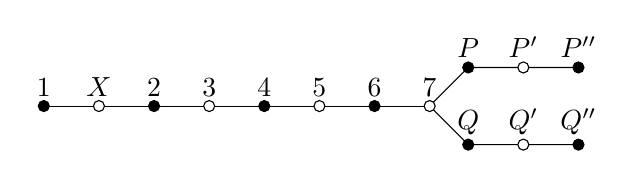
\begin{tikzpicture}[baseline=-1mm, scale=.7]
	\draw (0,0) -- (7,0);
	\draw (7,0)--(7.7,.7)--(9.7,.7);
	\draw (7,0)--(7.7,-.7)--(9.7,-.7);

	\filldraw              (0,0) node [above] {$1$} circle (1mm);
	\filldraw [fill=white] (1,0) node [above] {$X$} circle (1mm);
	\filldraw              (2,0) node [above] {$\JW{2}$}  circle (1mm);
	\filldraw [fill=white] (3,0) node [above] {$\JW{3}$}  circle (1mm);
	\filldraw              (4,0) node [above] {$\JW{4}$}  circle (1mm);
	\filldraw [fill=white] (5,0) node [above] {$\JW{5}$}  circle (1mm);
	\filldraw              (6,0) node [above] {$\JW{6}$}  circle (1mm);
	\filldraw [fill=white] (7,0) node [above] {$\JW{7}$}  circle (1mm);
	
	
	\filldraw              (7.7,.7) node [above] {$P$}  circle (1mm);
	\filldraw [fill=white] (8.7,.7) node [above] {$P'$}  circle (1mm);
	\filldraw              (9.7,.7) node [above] {$P''$}  circle (1mm);
	\filldraw              (7.7,-.7) node [above] {$Q$}  circle (1mm);
	\filldraw [fill=white] (8.7,-.7) node [above] {$Q'$}  circle (1mm);
	\filldraw              (9.7,-.7) node [above] {$Q''$}  circle (1mm);
\end{tikzpicture}$$

$$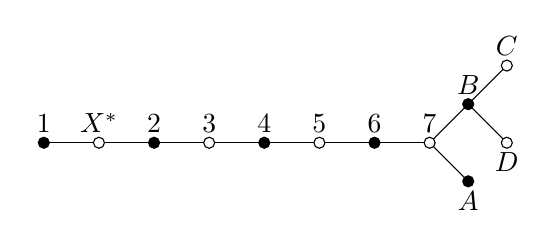
\begin{tikzpicture}[baseline=-1mm, scale=.7]
	\draw (0,0) -- (7,0);
	\draw (7,0)--(7.7,.7);
	\draw (7,0)--(7.7,-.7);
	\draw (7.7,.7)--(8.4,1.4);
	\draw (7.7,.7)--(8.4,0);

	\filldraw              (0,0) node [above] {$1$} circle (1mm);
	\filldraw [fill=white] (1,0) node [above] {$X^*$} circle (1mm);
	\filldraw              (2,0) node [above] {$\JW{2}$}  circle (1mm);
	\filldraw [fill=white] (3,0) node [above] {$\JW{3}$}  circle (1mm);
	\filldraw              (4,0) node [above] {$\JW{4}$}  circle (1mm);
	\filldraw [fill=white] (5,0) node [above] {$\JW{5}$}  circle (1mm);
	\filldraw              (6,0) node [above] {$\JW{6}$}  circle (1mm);
	\filldraw [fill=white] (7,0) node [above] {$\JW{7}$}  circle (1mm);
	
	
	\filldraw              (7.7,.7) node [above] {$B$}  circle (1mm);
	\filldraw              (7.7,-.7) node [below] {$A$}  circle (1mm);
	\filldraw [fill=white] (8.4,1.4) node [above] {$C$}  circle (1mm);
	\filldraw [fill=white] (8.4,0) node [below] {$D$}  circle (1mm);
\end{tikzpicture}$$
\caption{The names for the minimal idempotents in $\cH_1(\Complex)$. Even vertices are shown as filled circles, and odd vertices are shown as hollow circles.  The convention for $\cH_0(\Complex)$ is the same but with fewer $\JW{i}$.}
\label{fig:naming}
\end{figure}

\begin{lem}
\label{lem:S2}%
The `one-click' rotation $\rho^{1/2}(S)$, which is an element of $\cH_\ell(k)_{n,-}$, satisfies
\begin{align}
\rho^{1/2}(S)^2 & = -i [2] \lambda_\ell (\check{r}^{1/2} - \check{r}^{-1/2}) \rho^{1/2}(S) - [2]^2 \lambda_\ell^2 \JW{n} \notag \\
	& =  (\check{r}-1) \rho^{1/2}(S) + \check{r} \JW{n}. \label{eq:rhoS2}
\end{align}
\end{lem}
\begin{proof}
Take the formula for $\rho^{1/2}(S)^2$ appearing in \cite[Theorem 3.9]{0909.4099},
% $$\rho^{1/2}(S)^2 = - \omega^{1/2} r^{1/2} (\check{r}^{1/2} - \check{r}^{-1/2}) \rho^{1/2}(S) + \omega^{-1} r \JW{n}.$$
and recall that the $S$ there is $\lambda_\ell^{-1}$ times our generator $S$, and that since we are working in the lopsided planar algebra, there is an additional factor of $[2]^{-1}$ with each occurrence of $\rho^{1/2}$. This factor arises because in the notation of \S \ref{sec:lopsided}, if the planar algebras from \cite{0902.1294, 0909.4099} are denoted $\cP$, we're looking at $\cP_{\sqrt{D_\ell}}$, and $\rho^{1/2}$ has a single critical point shaded above, which is a maximum.
 Thus we obtain
$$[2]^{-2} \lambda_\ell^{-2} \rho^{1/2}(S)^2 = - [2]^{-1} \lambda_\ell^{-1} \omega^{1/2} r^{1/2} (\check{r}^{1/2} - \check{r}^{-1/2})\rho^{1/2}(S) + \omega^{-1} r \JW{n}$$
and after setting $r=1$, $\omega = -1$, using the formula for $\lambda_\ell$ and rearranging, this becomes the desired formula.
% \begin{align*}
% $$\rho^{1/2}(S)^2 = - i [2] \lambda_\ell (\check{r}^{1/2} - \check{r}^{-1/2})\rho^{1/2}(S) - [2]^{2} \lambda_\ell^{2}  \JW{n}.$$
%\end{align*}
\end{proof}

\begin{lem}
\label{lem:idempotents1}
The idempotents $P$, $Q$, $A$ and $B$ in $\cH_\ell^p$ and $\cH_\ell^d$ are given by 
\begin{align}
P & = \frac{1}{2}\left(\JW{n} + \frac{1}{\lambda_\ell}S\right) \label{eq:P} \\
Q & = \frac{1}{2}\left(\JW{n} - \frac{1}{\lambda_\ell}S\right) \label{eq:Q} \\
A & = \frac{1}{\check{r}+1}\left(\JW{n}  + \rho^{1/2}(S)\right) \label{eq:A} \\
B & = \frac{1}{\check{r}+1}\left(\check{r} \JW{n} - \rho^{1/2}(S)\right) \label{eq:B}
\end{align}
\end{lem}
\begin{proof}
The formulas certainly define idempotents, according to the formulas in Lemma \ref{lem:S2} and in Definition \ref{def:pa}. Since $\frac{1}{2}\left(\JW{n} + \frac{1}{\lambda_\ell}S\right)+\frac{1}{2}\left(\JW{n} - \frac{1}{\lambda_\ell}S\right) = \JW{n}$, we know these formulas for $P$ and $Q$ actually define the corresponding idempotents. Note the symmetry between $P$ and $Q$: rescaling $S$ by $-1$ interchanges the formulas for the idempotents.
Since $\frac{1}{\check{r}+1}\left(\JW{n}  + \rho^{1/2}(S)\right) + \frac{1}{\check{r}+1}\left(\check{r} \JW{n} - \rho^{1/2}(S)\right) = \JW{n}$, these formulas are indeed the idempotents $A$ and $B$; you can check which is which by taking the trace.
\end{proof}

\begin{lem}
\label{lem:idempotents2}
The remaining idempotents on the principal graph are given by 
\begin{align}
P' & = P \tensor X - \frac{2[n]}{[2][n+1]} \left((P \tensor X) \circ e_n \circ (P \tensor X)\right) \label{eq:P'} \displaybreak[1]\\
Q' & = Q \tensor X - \frac{2[n]}{[2][n+1]} \left((Q \tensor X) \circ e_n \circ (Q \tensor X)\right) \label{eq:Q'} \displaybreak[1] \\
P'' & = P' \tensor X^* -  \frac{[2][n+1]}{[n+2]-[n]} \left((P' \tensor X^*) \circ e_{n+1} \circ (P' \tensor X^*)\right) \label{eq:P''} \displaybreak[1] \\
\intertext{and}
Q'' & = Q' \tensor X^* -  \frac{[2][n+1]}{[n+2]-[n]} \left((Q' \tensor X^*) \circ e_{n+1} \circ (Q' \tensor X^*)\right).  \label{eq:Q''} 
\end{align}
\end{lem}
\begin{proof}
We know from the principal graph that $P \tensor X \iso \JW{n-1} \directSum P'$
We claim that the second term in the right hand side of Equation \eqref{eq:P'} is the projection onto $\JW{n-1}$, and so the difference is exactly $P'$. In fact, if the second term is a projection at all it must be equivalent to $\JW{n-1}$ as it factors through $n-1$ strands. The partial trace of $P$ is 
$$\ptr{P} = \frac{[2][n+1]}{2[n]} \JW{n-1}$$
and an easy calculation gives the result. An identical argument for $Q$ instead of $P$ gives Equation \eqref{eq:Q'}.

Equations \eqref{eq:P''} and \eqref{eq:Q''} follow similarly. We use that fact that $P' \tensor X^* \iso P \directSum P''$, and calculate $$\ptr{P'} = \left(1-\frac{2[n]}{[2][n+1]}\right) P = \frac{[n+2]-[n]}{[2][n+1]} P$$ from Equation \eqref{eq:P'}. Computing the square of the second term in Equation \eqref{eq:P''} confirms that it is a projection, and gives the result. The analogous considerations for $Q'$ instead of $P'$ give Equation \eqref{eq:Q''}.
\end{proof}

\begin{lem}
\label{lem:idempotents3}%
The idempotents $C$ and $D$ on the dual principal graph are given by
\begin{align}
C & = \rho^{n/2}(P') \label{eq:C} \\
\intertext{and}
D & = \rho^{n/2}(Q'). \label{eq:D}
\end{align}
\end{lem}
\begin{proof}
The idempotents $C$ and $P'$ are dual, as are $D$ and $Q'$.
\end{proof}

The coefficients appearing in Equations \eqref{eq:P} and \eqref{eq:Q} lie in $\Rational(\lambda_\ell)$ while the coefficients in Equations \eqref{eq:A} through \eqref{eq:D} all lie in $\Rational(D_\ell)$.

This planar algebra gives a possibly incomplete rational form for both even parts over $\Rational(D_\ell)$.  Since all of the projections in the dual even part lie in $\Rational(D_\ell)$ we have constructed a complete rational form for the dual even part in $\Rational(D_\ell)$.  Finally, since all of the projections in the principal even part lie in $\Rational(\lambda_\ell)$ we have a complete rational form for the principal even part over $\Rational(\lambda_\ell)$.
